\documentclass{../zkdl-presentation-template}

\title[Криптографія]{\textbf{Практичне №9.Криптосистеми Rabin. ZKP протоколи.}}

\date{2.12.2025}


\begin{document}
    \frame{
        \titlepage
    }
  
    \begin{frame}{Plan}
        \tableofcontents
    \end{frame}

%-----------------------------------------------
\section{Криптоаналіз шифрів}
%-----------------------------------------------
\begin{frame}{Задачі}
    \begin{block}{}
        1. Покажіть, що функція RSA зберігає символ Якобі \\
        2. Покажіть, що при $e=\frac{\phi(n)}{2}+1$ функція RSA перетворюється на тотожню.
        
\includegraphics[width=1\linewidth]{2-crypto-sym/images/cells.png}
    \end{block}
\end{frame}
%-----------------------------------------------
\section{Криптосистема Rabin}
%-----------------------------------------------
\begin{frame}
    \frametitle{Протокол}
        \begin{gather*}
            x^2\equiv a \text{ mod }n, \quad n=p\cdot q 
        \end{gather*}
            \begin{align*}
         \left\{ \begin{array}{r}
x^2= a \text{ mod } p, \left(\frac{a}{p}\right)=1  \\ 
x^2=a \text{ mod } q, \left(\frac{a}{q}\right)=1
\end{array}\right.
    \end{align*}
    \begin{columns}[c] % [c] вирівнювання по центру вертикалі
          \column{0.5\textwidth}
          \begin{align*}
\left\{ \begin{array}{r}
x=\pm \sqrt{a} \text{ mod } p  \\ 
x=\pm \sqrt{a} \text{ mod } q 
\end{array}\right.
\end{align*}
\column{0.5\textwidth}
\begin{align*}
\left\{ \begin{array}{r}
x=\pm x_p \text{ mod } p  \\ 
x=\pm x_q \text{ mod } q 
\end{array}\right.
\end{align*}
      \end{columns}
      \begin{figure}
          \centering
          
\includegraphics[width=1\linewidth]{2-crypto-sym/images/cells_small.png}
      \end{figure}
\end{frame}
%-----------------------------------------------------------
\begin{frame}{ЦП Rabin}
    \begin{figure}
        \centering
        
\includegraphics[width=1\linewidth]{2-crypto-sym/images/cells.png}
    \end{figure}
\end{frame}
%-----------------------------------------------------------
\section{Протоколи доведення без розголошення}
%-----------------------------------------------------------
\begin{frame}{Що таке ZKP?}
    \begin{figure}
        \centering
        
\includegraphics[width=1\linewidth]{9-crypto-practice/images/I-KNOW-THEY-KNOW-BUT-I-DONT-KNOW-WHAT-THEY-KNOW-meme.jpg}
    \end{figure}
\end{frame}

    \begin{frame}{Класичні Доведення}
        \begin{columns}
            % Description
            \begin{column}{0.6\textwidth}
                \begin{itemize}
                    \item Перші доведення, з якими ви, ймовірно,
                    стикалися, були \textbf{геометричними доведеннями}.
                    \item Вам давалися \textbf{аксіоми}, і ви могли
                    довести певні \textbf{твердження} $\mathbbm{x}$,
                    використовуючи їх. \item Доведення $\pi$ — це
                    послідовність логічних кроків, які доводять $\mathbbm{x}$.
                    По суті, у вас є свідок $\mathbbm{w}$, який доводить
                    твердження. \item Ваш вчитель — це
                    \textbf{верифікатор} $\mathcal{V}$, який перевіряє ваше
                    доведення, тоді як ви — \textbf{доказувач} $\mathcal{P}$.
                    \item Це \textbf{класичне доведення}, і в певному
                    сенсі \textbf{неінтерактивне}.
                \end{itemize}
            \end{column}
            % Column 2
            \begin{column}{0.4\textwidth}
                \begin{figure}
                \centering
                    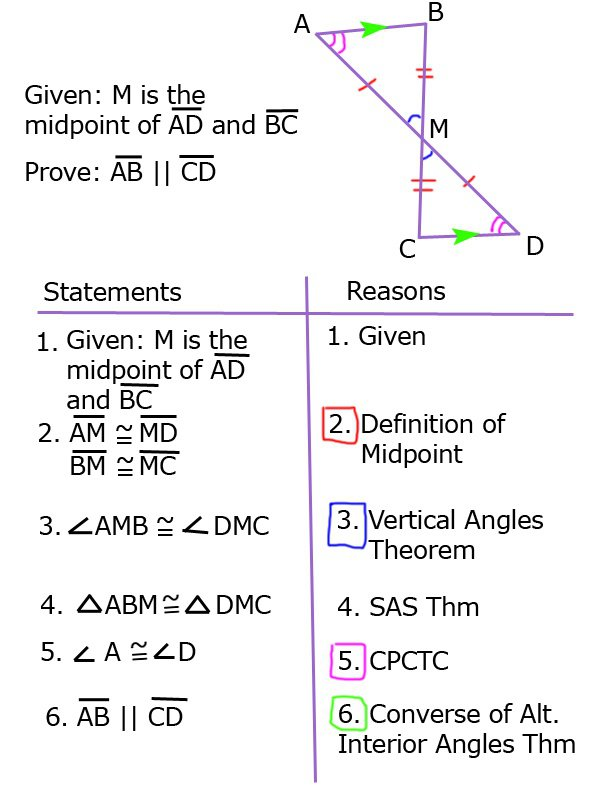
\includegraphics[width=1.0\textwidth]{9-crypto-practice/images/geometry-proof.jpg}
                    \caption{Геометричне доведення.}
                \end{figure}
            \end{column}
            \end{columns}
    \end{frame}
    
    \begin{frame}{Найпростіша постановка задачі}
        \begin{itemize}
            \item У нас є \textbf{доказувач} $\mathcal{P}$ і
            \textbf{верифікатор} $\mathcal{V}$. 
            \item Доказувач
            $\mathcal{P}$ хоче довести певне твердження $\mathbbm{x}$
            верифікатору. 
            \item Доказувач $\mathcal{P}$ має
            \textbf{свідка} $\mathbbm{w}$, який містить всю необхідну інформацію
            для доведення $\mathbbm{x}$. Він надсилає $\pi$ як доведення.
            \item Верифікатор $\mathcal{V}$ хоче переконатися, що
            $\mathbbm{x}$ є істинним.
        \end{itemize}

        \begin{figure}
            \centering
            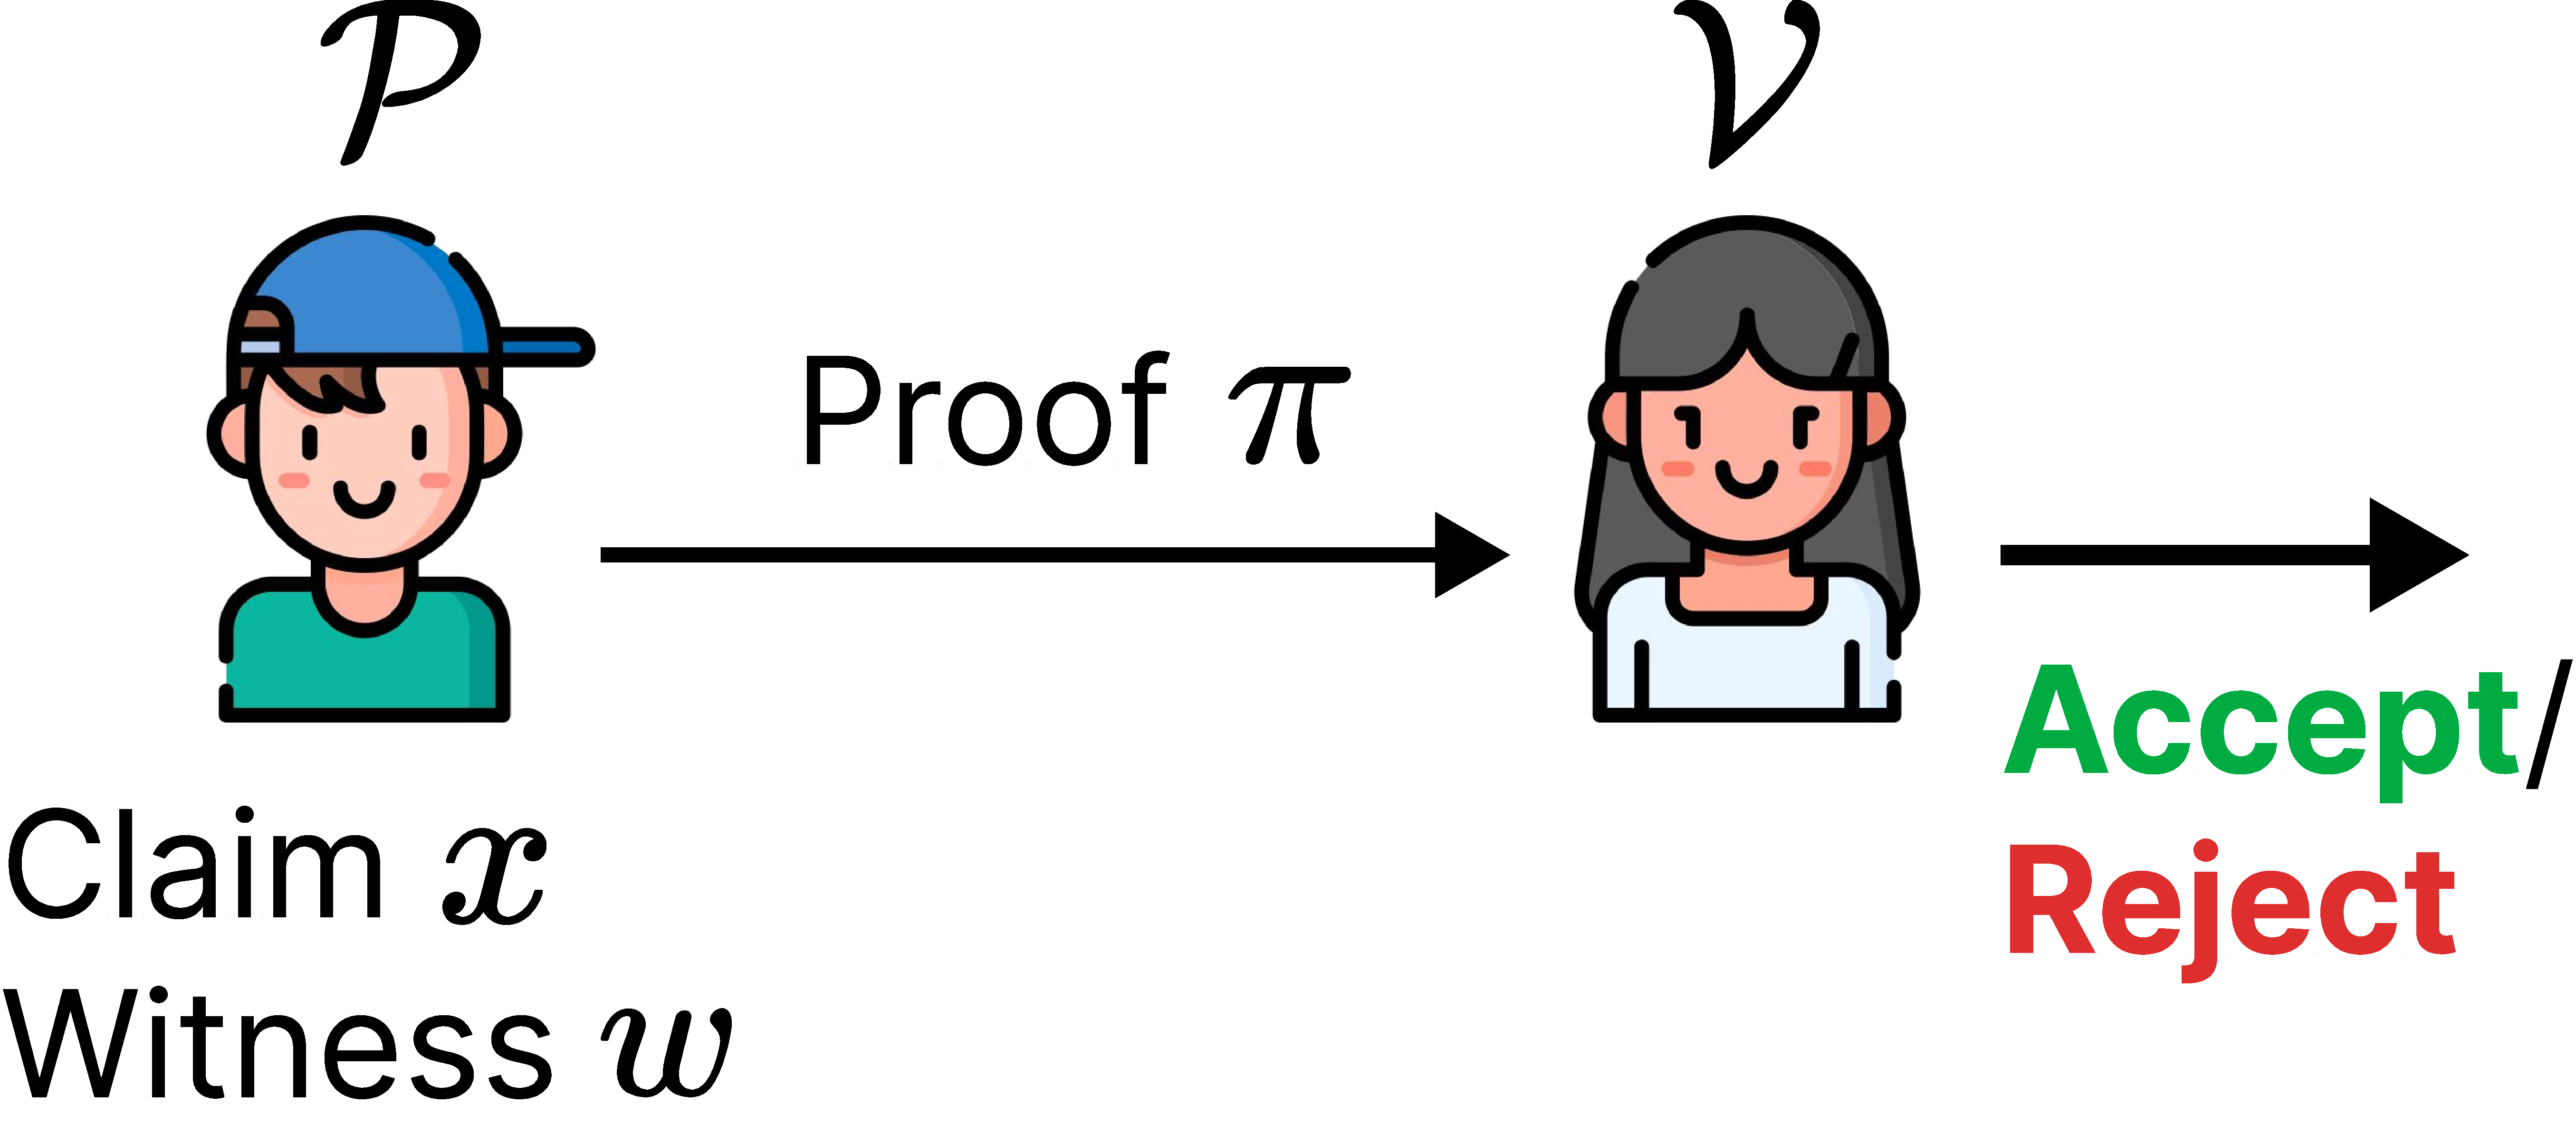
\includegraphics[width=0.7\textwidth]{9-crypto-practice/images/setup.pdf}
            \caption{Типова постановка для криптографічних доведень.}
        \end{figure}
    \end{frame}

        \begin{frame}{Мета сучасних ZK протоколів}
        \begin{itemize}[label=\cmark]
            \item \textbf{Повнота:} Якщо $\mathbbm{x}$ істинне, $\pi$ доводить твердження.
            \item \textbf{Коректність (Soundness):} Якщо $\mathbbm{x}$ хибне, доказувач $\mathcal{P}$ не повинен мати змоги переконати верифікатора $\mathcal{V}$ за допомогою будь-якого $\pi^*$.
            \item \textbf{Нульове знання:} $\pi$ нічого не розкриває про $\mathbbm{w}$.
            \item \textbf{Аргумент знання:} Іноді доказувач $\mathcal{P}$ повинен переконати верифікатора $\mathcal{V}$, що, крім того, що $\mathbbm{x}$ є істинним, він \textbf{знає} свідка $\mathbbm{w}$. Ми це продемонструємо пізніше. 
            \item \textbf{Стислість:} Доведення має бути коротким, в ідеалі полілогарифмічним від розміру твердження ($|\pi| = \mathsf{polylog}(|\mathbbm{x}|)$) + швидка верифікація.
            \item \textbf{Арифметизація:} Нам потрібно перетворити твердження $\mathbbm{x}$ у певну алгебраїчну форму, зробивши її універсальною.
        \end{itemize}
    \end{frame}

    \begin{frame}{Приклад для демонстрації мети}
        \begin{example}
            Дано геш-функцію $\mathcal{H}: \{0,1\}^* \to \{0,1\}^{\ell}$, $\mathcal{P}$ хоче переконати $\mathcal{V}$, що він знає прообраз $x \in \{0,1\}^*$ такий, що $\mathcal{H}(x) = y$.
            \begin{itemize}
                \item \textbf{Нульове знання:} Доказувач $\mathcal{P}$ не хоче розкривати \textit{нічого} про прообраз $x$ верифікатору $\mathcal{V}$.
                \item \textbf{Аргумент знання:} Доведення того, що $y$ має прообраз, є марним: потрібно показати саме \textbf{знання} $x \in \{0,1\}^*$.
                \item \textbf{Стислість:} Якщо для обчислення хеш-функції потрібно $n$ операцій, доведення має бути \textbf{значно} коротшим за $n$ операцій. \textbf{Сучасний рівень}: розмір $O(\mathsf{polylog}(n)) = O((\log n)^{\gamma})$. Час верифікації також зазвичай полілогарифмічний (або навіть $O(1)$ у деяких випадках).
            \end{itemize}
        \end{example}
    \end{frame}
        
        \begin{frame}{Мова}
        \begin{definition}[Відношення]
            Дано дві множини $\mathcal{X}$ та $\mathcal{Y}$, \textbf{відношення} — це $\mathcal{R} \subseteq \mathcal{X} \times \mathcal{Y}$.
            \begin{itemize}
                \item $\mathcal{X}$ — це зазвичай множина \textbf{тверджень}.
                \item $\mathcal{Y}$ — це множина \textbf{свідків}.
            \end{itemize}
        \end{definition}

        \begin{definition}[Мова істинних тверджень]
            Нехай $\mathcal{R} \subseteq \mathcal{X} \times \mathcal{Y}$ — це відношення. Ми кажемо, що твердження $x \in \mathcal{X}$ є \textbf{істинним} твердженням, якщо $(x,y) \in \mathcal{R}$ для деякого $y \in \mathcal{Y}$, інакше твердження називається \textbf{хибним}. Ми визначаємо $\mathcal{L}_{\mathcal{R}}$ (мову над відношенням $\mathcal{R}$) як множину всіх істинних тверджень, тобто:
            \begin{equation*}
                \mathcal{L}_{\mathcal{R}} = \{ x \in \mathcal{X}: \exists y \in \mathcal{Y} \; \text{такий, що} \; (x,y) \in \mathcal{R} \}.
            \end{equation*}
        \end{definition}
    \end{frame}

    \begin{frame}{Приклад мови №1: Напівпрості числа}
        \begin{example}[Добуток двох простих чисел]
            \textbf{Твердження:} число $n \in \mathbb{N}$ є добутком двох простих чисел $w = (p,q) \in \mathbb{N} \times \mathbb{N}$. \textbf{Відношення} задається як:
            \begin{equation*}
                \mathcal{R} = \{ (n, (p, q)) \in \mathbb{N} \times \mathbb{N}^2: n = p \cdot q \; \text{де $p,q$ — прості числа} \}
            \end{equation*}

             У цьому конкретному випадку \textbf{мова істинних тверджень}:
            \begin{equation*}
                \mathcal{L}_{\mathcal{R}} = \{n \in \mathbb{N}: \exists w=(p,q) \; \text{є простими такими, що}\; n = p\cdot q\}
            \end{equation*}

            \begin{itemize}
                \item \textcolor{green!50!black}{\textbf{Дійсний свідок №1:}} $n=15 \in \mathcal{L}_{\mathcal{R}}$. Свідок: $w=(3,5)$.
                \item \textcolor{red!80!black}{\textbf{Недійсний свідок:}} $n=16 \not\in \mathcal{L}_{\mathcal{R}}$. Немає дійсного свідка.
                \item \textcolor{green!50!black}{\textbf{Дійсний свідок №2:}} $n=50252009 \in \mathcal{L}_{\mathcal{R}}$. Свідок: $w=(5749,8741)$.
            \end{itemize}
        \end{example}
        \vspace{-10px}
        \textcolor{purple}{\textbf{Питання:}} Чи є $n=27$ істинним твердженням? $n=26$?
    \end{frame}

    \begin{frame}{Приклад мови №2: Квадратний корінь}
        \begin{example}
            \textbf{Твердження}: число $x \in \mathbb{Z}_N^{\times}$ є \textbf{квадратичним лишком} за модулем $N$: $(\exists w \in \mathbb{Z}_N^{\times}): \{x \equiv w^2 \pmod{N}\}$.

            \textbf{Відношення}: $\mathcal{R} = \{ (x, w) \in (\mathbb{Z}_N^{\times})^2: x \equiv w^2 \pmod{N} \}$. 

            \textbf{Мова:} $\mathcal{L}_{\mathcal{R}} = \{x \in \mathbb{Z}_N^{\times}: \exists w \in \mathbb{Z}_N^{\times} \; \text{такий, що} \; x \equiv w^2 \pmod{N}\}$. 

            \textbf{Приклади} для $N=7$: а) 4, б) 3.
            \begin{figure}
                \centering
                
\includegraphics[width=1\linewidth]{2-crypto-sym/images/cells_small.png}
            \end{figure}
        \end{example}
    \end{frame}

    \begin{frame}{Sigma protocol}
    \begin{block}{Означення.}
        $\Sigma$-protocol для ефективно обчислювального відношення $R \subseteq \{0, 1\}^* \{0, 1\}^*$ -- це 3-раундовий протокол для якого виконуються наступні властивості:
    \begin{itemize}
        \item $\Sigma$-структура. Доказувач перший надсилає комітмент, далі верифікатор надсилає деякий згенерований челендж і доказувач повинен надати послідовну відповідь.
        \item Функціональність. Протокол є взаємодією чесного доказувача $P(sk)$ та верифікатора $V(pk)$, що завжди приймає доказ якщо $(sk, pk)\in \mathcal{R}$. 
    \end{itemize}
    \end{block}
    \end{frame}

    \begin{frame}{Sigma protocol}
         \begin{figure}
        \centering
        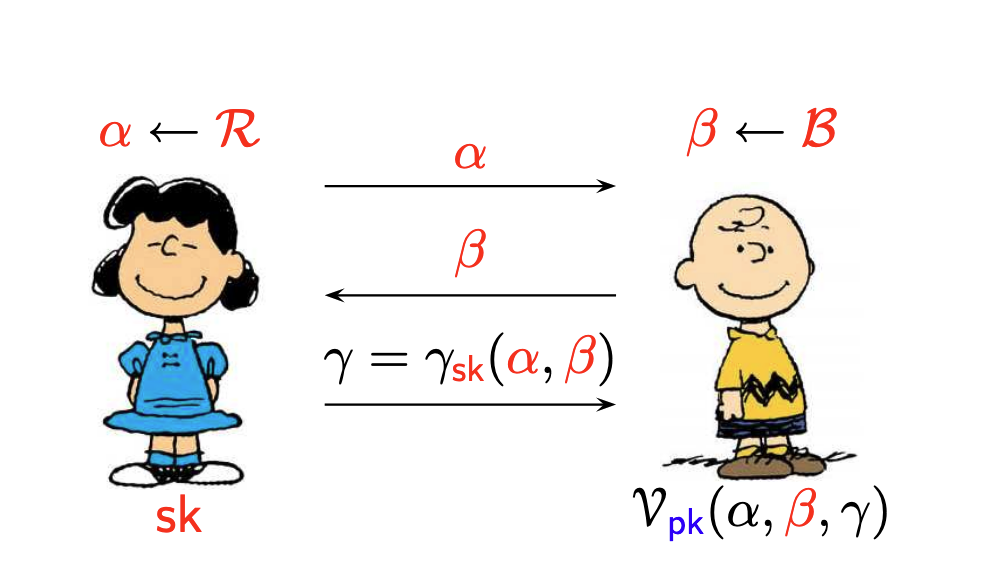
\includegraphics[width=1\linewidth]{9-crypto-practice/images/Sigma_new.png}
    \end{figure}
    \end{frame}

    \begin{frame}{Неінтерактивність та евристика Фіат-Шаміра}
        \begin{block}{Твердження}
            \textbf{Будь-який} інтерактивний протокол з публічною монетою можна перетворити на неінтерактивний протокол з публічною монетою зі збереженням повноти, обґрунтованості та нульового знання за допомогою випадкового оракула.
        \end{block}

        Одне з таких перетворень називається \textbf{евристикою Фіата-Шаміра}. Ідея:
        \begin{enumerate}
            \item Якщо все, що робить $\mathcal{V}$, — це надсилання рівномірно випадкових значень, то навіщо нам інтеракція? 
            \item Замість того, щоб $\mathcal{V}$ надсилав випадкові значення, доказувач повинен мати можливість генерувати їх самостійно, але він не повинен знати випадковість заздалегідь.
            \item Отже, ми можемо замінити повідомлення верифікатора хешем (випадковим оракулом) всієї попередньої розмови.
        \end{enumerate}
    \end{frame}

    
    \begin{frame}{Неінтерактивний Sigma protocol}
        \begin{figure}
            \centering
            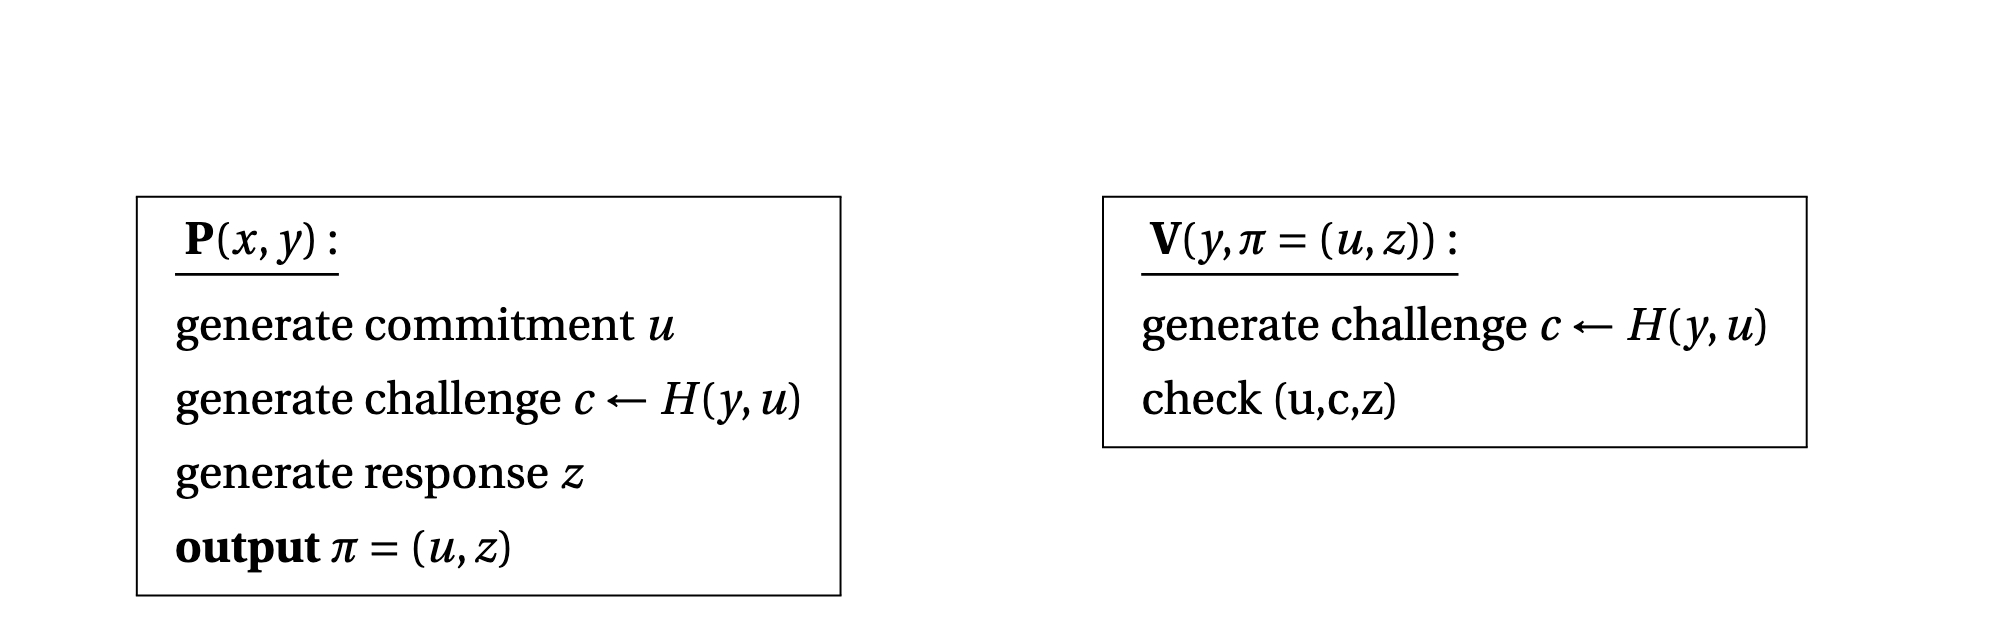
\includegraphics[width=1\linewidth]{9-crypto-practice/images/Sigma_nonint.png}
        \end{figure}
    \end{frame}

    \begin{frame}{Приклад}
    \begin{block}{}
        Покажіть, що Боб може довести Алісі, що володіє секретом $x=3$, не розкриваючи його. Для цього використайте $\Sigma$-протокол в налаштуванні Шнорра, де $p=19, g=2,r=7$, а челендж що надіслала Аліса $c=5$.
        \begin{figure}
            \centering
            
\includegraphics[width=0.9\linewidth]{2-crypto-sym/images/cells.png}
        \end{figure}
    \end{block}
        
    \end{frame}
    \begin{frame}[plain, standout]
    \begin{figure}
        \centering
        
\includegraphics[width=0.9\linewidth]{Cryptocats.jpg}
        \label{fig:placeholder}
    \end{figure}
    \centering
    \LARGE
    \textbf{Питання?} \\

    \vspace{0.2cm} \Huge \ding{170} \large \\

  \end{frame}
\end{document}